\chapter{bb-tagging Scale Factors for W jets in $t\bar{t}$ Events}

The $b\bar{b}$-tagger has a non-zero probability to tag an AK8 jet from a boosted W boson as arising from a two b quark decay. This \textit{mistag} rate can, in principle, be different in simulation compared to data. Depending on the use, it may be necessary to apply \textit{scale factors} to the simulation to correct for this difference.

To calculate the mistag rates, we obtain a sample of W jets is by selecting semi-leptonic $t\bar{t}$ events. To select these events, we require a single muon ($p_{T}>50\,\textrm{GeV}$, $|\eta|<2.1$)  within close proximity ($\delta\phi < \frac{2}{3}\pi$) of a b-tagged AK4 jet. Opposite this muon ($\delta\phi<\frac{2}{3}\pi$) we require a single AK8 jet ($p_{T}>250 GeV$, $|\eta|<2.4$). The jet is required to have mass $50 < m < 200\,\textrm{GeV}$. This decay is illustrated on the right-side of Figure~\ref{fig:ttbar}. 

Afte
The sample is found to be very pure, as evidence in the mass distribution with a peak near $m_{W} = 80.385\,\textrm{GeV}$. A small contribution at $m_{top}=172.44\,\textrm{GeV}$ is seen in the tail - contamination from boosted top quarks decaying to W bosons and b jets which are collinear resulting in single jet reconstruction.

\begin{figure}[hbp!]
\centering
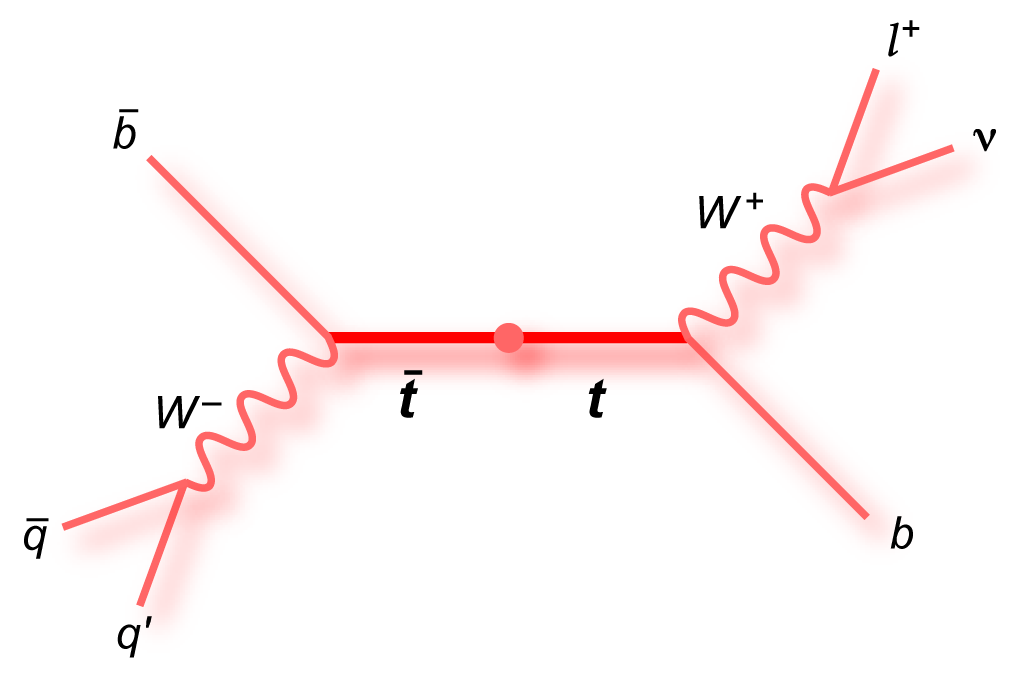
\includegraphics[width=0.4\textwidth]{figs/feynman_ttbar_ljets_beamline.png}
\caption[A  diagram of a $t\bar{t}$ event in the center-of-mass frame.]{A  diagram of a $t\bar{t}$ event in the center-of-mass frame \cite{ttbar}.}
\label{fig:ttbar}
\end{figure}

This selection provides a relatively pure sample of W boson jets.

\begin{figure}[hbp!]
\centering
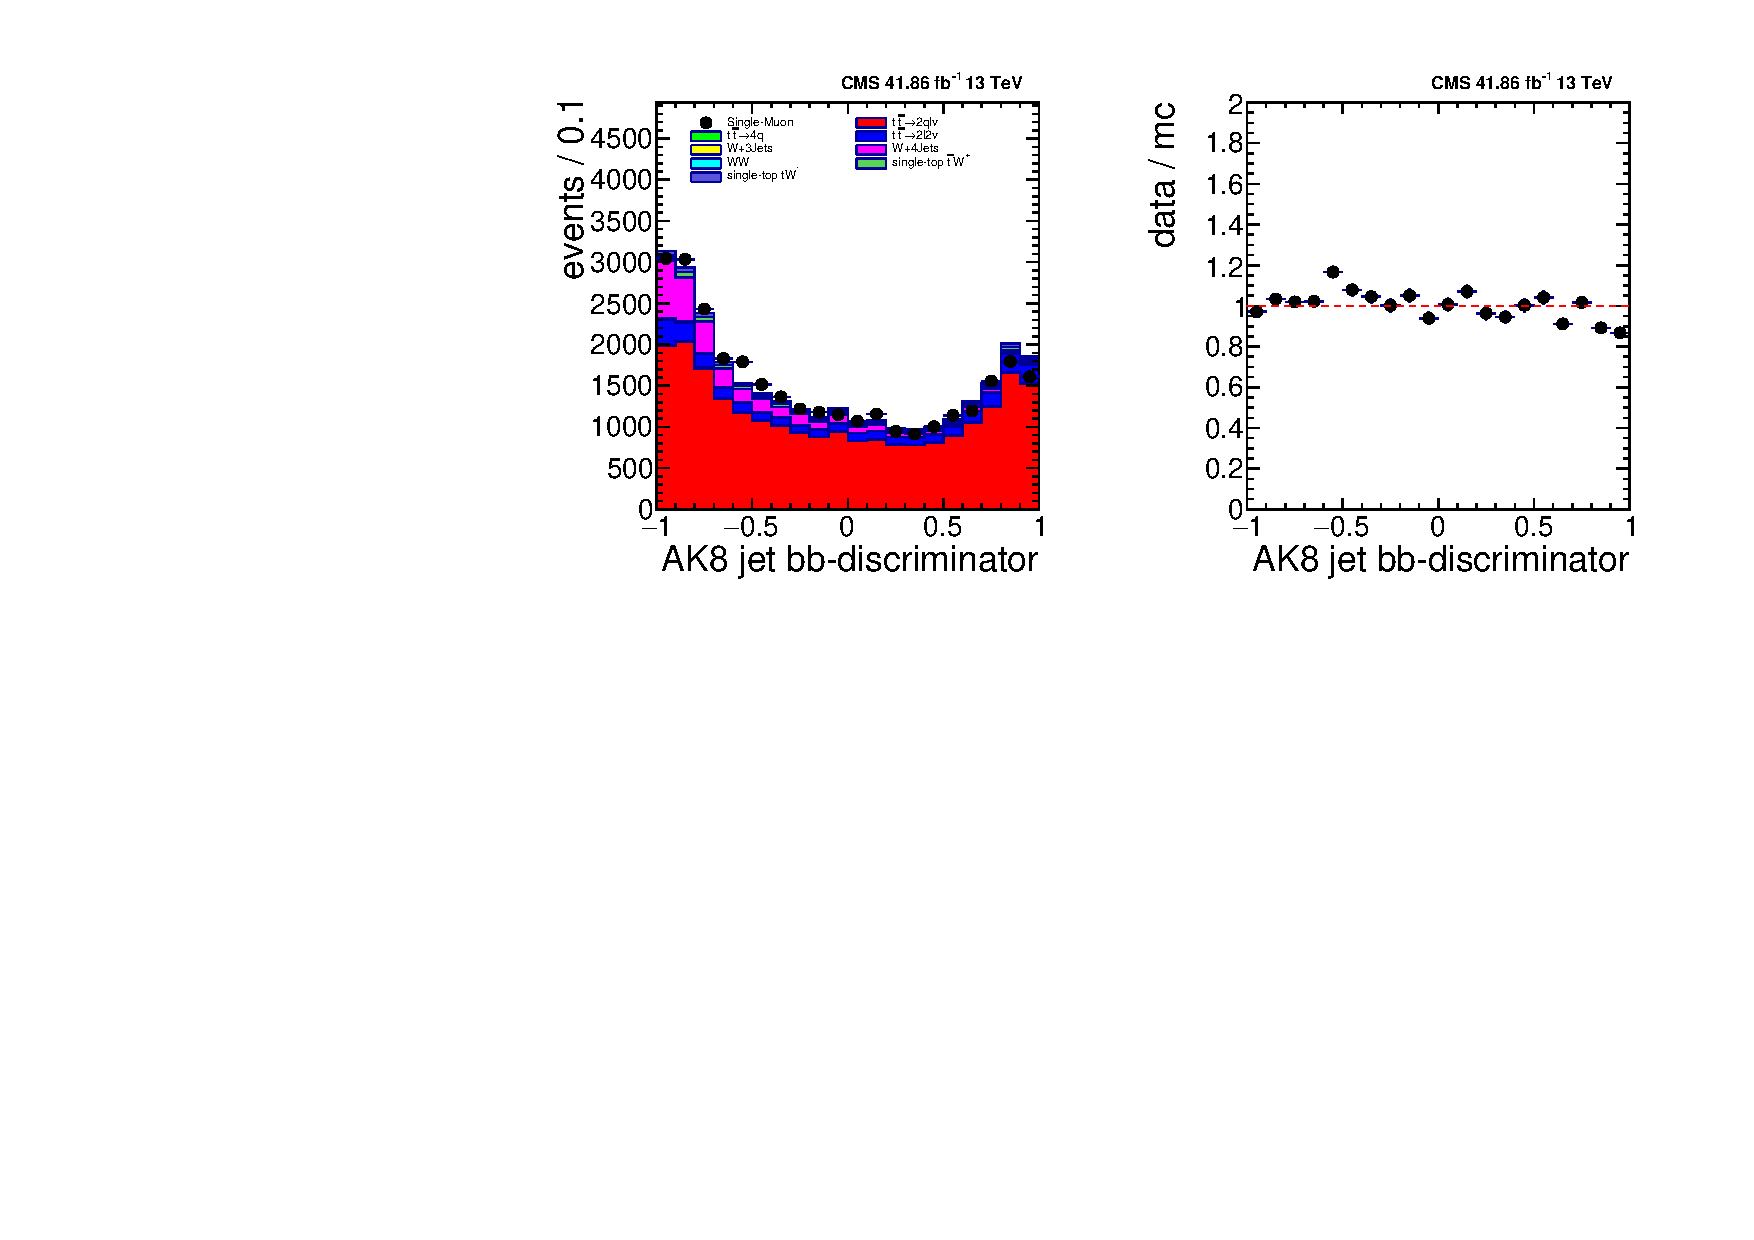
\includegraphics[width=0.75\textwidth]{figs/datamccomparisons_hadJetAK8_disc.pdf}
\caption{Comparisons of the $b\bar{b}$-tagging discriminator in data and simulation.}
\label{fig:disc}
\end{figure}

\begin{figure}[hbp!]
\centering
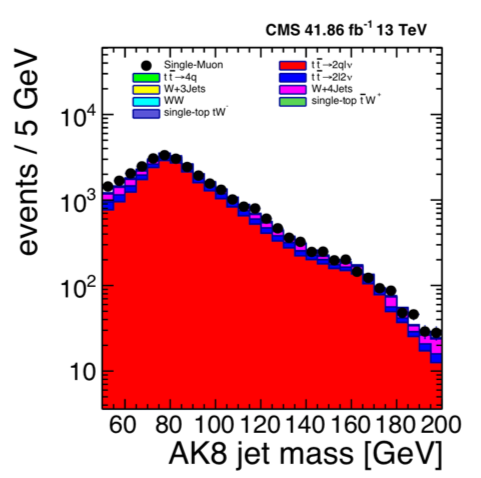
\includegraphics[width=0.375\textwidth]{figs/ak8jetmass.png}
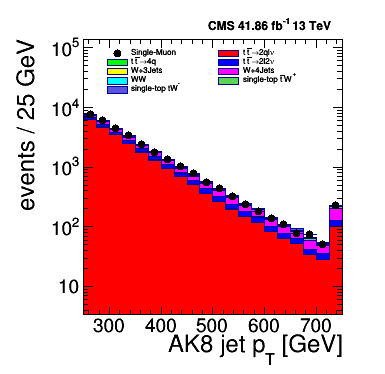
\includegraphics[width=0.375\textwidth]{figs/ak8jetpt.png}
\caption{W jet mass and $p_{T}$ in data and simulation.}
\label{fig:disc}
\end{figure}

\begin{equation}
\epsilon_{mc} = \frac{ N_{b\bar{b}-tagged}^{sig, mc} } { N^{sig, mc} }, \hspace{1cm}
\epsilon_{data} = \frac{N_{b\bar{b}-tagged}^{data}-N_{b\bar{b}-tagged}^{bkg, mc}}{N^{data} - N^{bkg, mc}}, \hspace{1cm}
sf = \frac{\epsilon_{data}} {\epsilon_{mc}}
\end{equation}

\begin{table}[hbp!]
\centering
\caption{Mistag rates in data and simulation, inclusive in $p_{T}$.}
\label{tab:mistag}
\begin{tabular}{c|cc}
\hline\hline
working point & data & mc\\
\hline
disc $>$ 0.3 & 0.326 $\pm$ 0.003 & 0.340 $\pm$ 0.003 \\
disc $>$ 0.6 & 0.219 $\pm$ 0.003 & 0.236 $\pm$ 0.002 \\
disc $>$ 0.8 & 0.122 $\pm$ 0.002 & 0.138 $\pm$ 0.002 \\
disc $>$ 0.9 & 0.058 $\pm$ 0.001 & 0.067 $\pm$ 0.001 \\
\hline\hline
\end{tabular}
\end{table}

\begin{table}[hbp!]
\centering
\caption{Summary of scale factors for $b\bar{b}$-tagging W jets in $t\bar{t}$ events.}
\label{tab:sf}
\begin{tabular}{l|lll}
\hline\hline
working point & $250 < p_{T} < 350\,\textrm{GeV}$ & $350 < p_{T} < 430\,\textrm{GeV}$ & $p_{T}>430\,\textrm{GeV}$\\
\hline
disc $>$ 0.3 & 0.939$\pm$0.026 & 1.007$\pm$0.055 & 0.996$\pm$0.079/0.079 \\
disc $>$ 0.6 & 0.922$\pm$0.027 & 0.967$\pm$0.057 & 0.902$\pm$0.082/0.082  \\
disc $>$ 0.8 & 0.875$\pm$0.030 & 0.939$\pm$0.063 & 0.893$\pm$0.090/0.090  \\
disc $>$ 0.9 & 0.875$\pm$0.030 & 0.939$\pm$0.063 & 0.893$\pm$0.090/0.090  \\
\hline\hline
\end{tabular}
\end{table}
